% !TEX encoding = UTF-8
% !TEX TS-program = pdflatex
% !TEX root = ../tesi.tex

%**************************************************************
\chapter{Descrizione dello stage}
\label{cap:descrizione-stage}
%**************************************************************

\intro{In questo capitolo andrò a descrivere i principali aspetti che sono stati trattati durante lo stage}\\

%**************************************************************
\section{Introduzione al progetto}
Visto in scala più ampia, il progetto finale risulterà una rivisitazione di Bipod, un applicativo di Siav, in ambito process mining, utilizzato come gestore di processi aziendali.
Tale software, dopo averlo provato con mano, risulta funzionale in ogni sua parte, anche se la sua struttura risulta poco estendibilea. Per questo motivo mi è stato proposto di sviluppare una parte di software che si andrà poi ad integrare con il nuovo applicativo che adrà a rimpiazzare l'attuale esistente.
Nello specifico le richieste a cui ho fatto fronte sono state le seguenti:
\begin{itemize}
	\item Libreria di process mining per filtraggio su log degli eventi.
	\item Interfaccia fronted tenendo come punto di riferimento il vecchio applicativo.
	\item Stub per verificare il correntto comportamento dell'interfaccia di filtraggio
\end{itemize}
\section{Studio tecnologico}
\subsection{Ambito process mining}
Fin dal primo momento sono stato formato dal tutor tramite videolezioni e l'utilizzo di alcuni tool di process mining, cercando di entrare a fondo nel contensto dell'analisi dei processi.
I software utilizzati sono stati i seguenti:
\begin{itemize}
	\item Bipod : Software proprietario di \textit{Siav} per la gestione ed il miglioramento di processi aziendali.
	\item ProM : Software di mining, modulare e flessibile sviluppato da \textit{Eindhoven University of Technology}
	\item Disco: Software leader nel settore del process mining sviluppato da \textit{Fluxicon}
\end{itemize}
\subsection{Framework java per applicazione cloud}
Un framework si definisce come un set di istruzioni pre-compilato, che fornisce funzionalità
generiche e che possono essere adattate alle necessità degli utenti. 
L’utilizzo dei framework garantisce al programmatore un ingente
risparmio di tempo e la certezza di utilizzare strumenti standard, dovuto ad un way
of working solido che aderisce alle best practice. Nel mio caso tale nozione è stata fondamentale per lo sviluppo della libreria, garantendomi una buona solidità e mantanibilità del codice
\subsection{OpenXes}
OpenXes è una libreria di process mining aderente allo standard XES. In questa libreria i log sono visti come file ".xes". Il log è rappresentato da una classe denominata XLog, contente al suo interno una lista di tracce denominata XTrace, che rappresenta un singolo processo all'interno del log. Ogni XTrace contiene la lista di eventi che formano quel dato processo. La classe che rappresenta il singolo evento è denominata Xevent
\begin{figure}[!h] 
	\centering 
	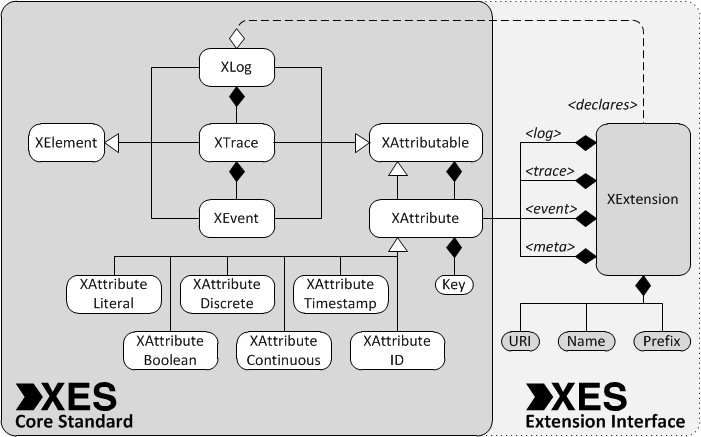
\includegraphics[width=0.9\columnwidth]{openxes} 
	\caption{Diagramma dei package dello standard openXes}
\end{figure}
\subsection{Docker}
Docker è una piattaforma che automatizza il deployment di applicazioni all'interno di contenitori software tramite virtualizzazioni a livello di sistema operativo. Tali contenitori, aventi ognuno la propria logica ed implementazione, garantiscono funzionalità di isolamento rispetto agli altri. Lo studio di questa tecnologia non è stata approfondita a pieno in quanto, dopo la negoziazione dei requisiti, non vi è stata la necessità di entrare più nel dettaglio. È stata sufficente una infarinatura generale per poter comprendere l'architettura finale che presenterà il prodotto. 
\subsection{Web socket}
Web Socket è una tecnologia che fornisce canali di comunicazione bidirezionali attraverso una singola connessione. Questi canali sono sempre "aperti" durante tutto il lifecycle dell'applicativo, effettuando richieste, e ricevento risposte in un unico canale. Tale tecnologia è stata concretizzata lato broswer avvalendosi della Liberia RxJS in modo da gestire sie le chiamate che gli eventi di ritorno. Per quanto riguarda il lato server, tramite l'implementazione di alcuni stub scritti in Python, è stato possibile gestire l'interfaccia in base ai messaggi ritorno inviati dallo stub.
\begin{figure}[!h] 
	\centering 
	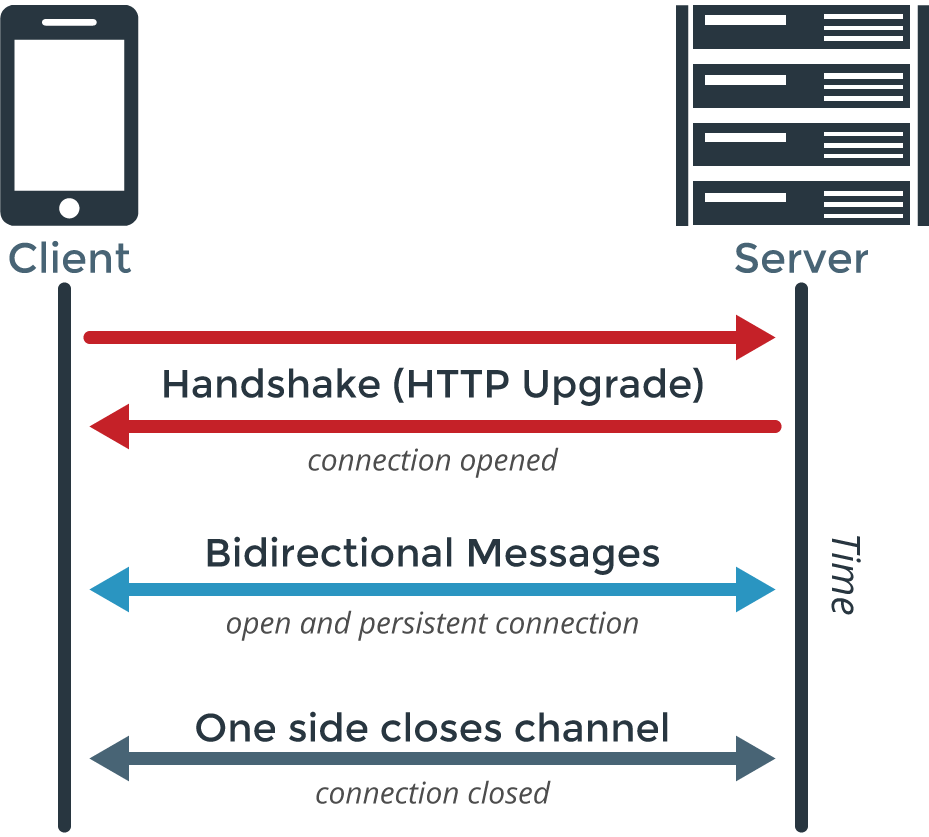
\includegraphics[width=0.6\columnwidth]{websocket} 
	\caption{Ciclo di vita di una connessione tramite websocket}
\end{figure}
\subsection {Angular}
Angular è una piattaforma opensource per lo sviluppo di web application scritto in TypeScript.
Una applicazione Angular può essere vista come un insieme di componenti visivi a sè stanti i quali occupano una porizione dell'intera applicazione. Ciascun componenete rappresenta un'entità configurabile e personalizzabile e può essere inserita all'interno di altri componenti.
\begin{figure}[!h] 
	\centering 
	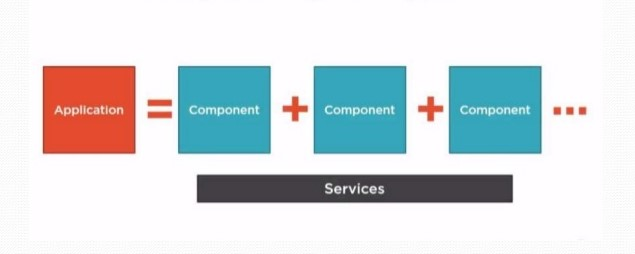
\includegraphics[width=0.3\columnwidth]{angular} 
	\caption{Logo di Angular e TypeScript}
\end{figure}
\section{Analisi preventiva dei rischi}

Durante la fase di analisi iniziale sono stati individuati alcuni possibili rischi a cui si potrà andare incontro. Innanzitutto mi sono documentato sulle tipologie di filtraggio possibili dato un log degli eventi. Da qui, sotto consiglio del tutor, ho iniziato a studiare le librerie di process mining presenti all'interno del repository di ProM, un applicativo di process mining modulabile in cui è possibile l'integrazione con varie librerie. Tali librerie risultavano però scarsamente documentate, non aggiornate, e di difficile comprensione.\\

\begin{risk}{Reperimento package dal repository di ProM}
    \riskdescription{All'interno del repository di ProM sono presenti centinaia di librerie dedicate al process mining, quest'ultime però risultano scarsamente documentate e non aggiornate}
    \risksolution{la maggior parte delle librerie presenti fanno riferimento ad uno Standard denominato openXes, tale standard permette la rappresentazione delle principali strutture derivanti dai log degli eventi. Sono quindi partito da un progetto ex novo basandomi sullo standard sopracitato per la realizzazione della libreria}
\end{risk}

\begin{risk}{Reperimento dettagli implementativi di filtraggio}
	\riskdescription{Usando Bipod come riferimento ho discusso con il tutor in merito a tutte le possibili richieste di filtraggio che sarebbero state implementate. Ne è emerso che, sotto alcuni aspetti, alcune richieste saranno riviste e riscritte}
	\risksolution{Mi sono avvalso del software Disco, uno dei più noti tool di process mining per poter studiare il comportamento di tutte le richieste filtraggio all'interno di un log degli eventi, stilando una lista dettagliata dei possibili metodi che sarebbero serviti per ricorprire tutti requisiti concordati con il tutor.}
\end{risk}


%**************************************************************
\section{Requisiti e obiettivi}
I requisiti all'interno del progetto sono stati tracciati utilizzando come riferimento il vecchio applicativo Bipod e il software Disco. Da qui è stato possibile tracciare tutte le tipologie di filtraggio richieste ed il loro funzionamento:
\begin{itemize}
	\item Filtaggio per tempo : filtraggio di un log sulla base di attributi temporali
	\item Filtraggio per performance: filtraggio di un log sulla base della durata di un singolo evento, o sulla latenza tra due eventi
	\item Filtraggio per Attività di Inizio e Fine: filtraggio sulle tracce
\end{itemize}

%**************************************************************
\section{Pianificazione}